\documentclass[onlytextwidth]{beamer}
\usepackage[utf8]{inputenc}
\usepackage{microtype}
\usepackage{amsmath}
\usepackage{amssymb}
\usepackage[nomessages]{fp} %\FPeval{\var-name}{2*sin(pi/6)}
\usepackage{siunitx} %units in math. eg 20\milli\meter
\usepackage{yhmath} % for arcs, overparenth command
\usepackage{tikz} %graphics
\usetikzlibrary{quotes, angles}
%\usepackage{graphicx} already loaded by beamer class
%consider setting \graphicspath{{images/}}
%\parskip ?? to avoid paragraph indent
\usepackage{multicol} %may not need this package, just columns environment
\usepackage{venndiagram}

\subtitle[BECA]{Bronx Early College Academy}
\author[Huson]{Christopher J. Huson PhD}

\setbeamertemplate{headline}{\vskip2mm 
  BECA / \insertshortauthor \, / \inserttitle
  \hfill 
  \insertsection
  }

\title{Geometry Unit 1: Extra slides for Segments, Length, and Area}
\date{8-23 September 2022}

\begin{document}
\frame{\titlepage}

\section[Outline]{}
\frame{\tableofcontents}

\section{Extra 1.1 Isosceles triangle solving for length }

\begin{frame}{Diagrams and notation}
  What is shown in the diagram? Mark all that apply.
  \begin{enumerate}
    \item A rectangle
    \item An equilateral triangle
    \item An isosceles triangle
    \item A triangle that is neither isosceles nor equilateral
  \end{enumerate}
  \begin{center}
    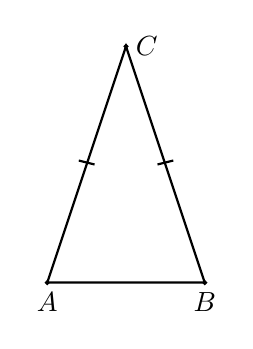
\begin{tikzpicture}[scale=0.5]
      \draw [thick](0,0)--(4,0)--(2,6)--(0,0);
      \draw [fill] (0,0) circle [radius=0.05] node[below]{$A$};
      \draw [fill] (4,0) circle [radius=0.05] node[below]{$B$};
      \draw [fill] (2,6) circle [radius=0.05] node[right]{$C$};
      \draw [thick] (0.8,3.1)--(1.2,3); %tick mark
      \draw [thick] (2.8,3)--(3.2,3.1); %tick mark
    \end{tikzpicture}
  \end{center}
\end{frame}

\begin{frame}{Isosceles triangle solving for length}
  \begin{block}{Do Now: Given $\overline{RST}$, $RS=3 \frac{2}{3}$, and $RT=9 \frac{1}{3}$. Find ${ST}$.}\vspace{0.5cm}
      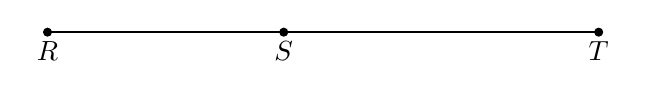
\begin{tikzpicture}
        \draw [-, thick] (0,0)--(7,0);
        \draw [fill] (0,0) circle [radius=0.05] node[below]{$R$};
        \draw [fill] (3,0) circle [radius=0.05] node[below]{$S$};
        \draw [fill] (7,0) circle [radius=0.05] node[below]{$T$};
      \end{tikzpicture}
  \end{block} \vspace{0.5cm}
\end{frame}

\begin{frame}{Isosceles triangle perimeter}
  Find the perimeter of the isosceles $\triangle ABC$, given $\overline{AC} \cong \overline{BC}$, $AB=7$, and $AC=10$\\[0.5cm]
  Show your work with an equation for full credit.\\
    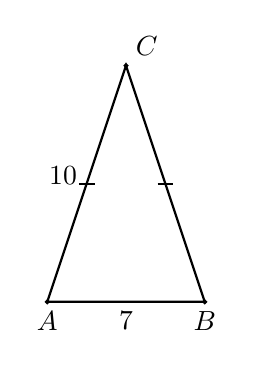
\begin{tikzpicture}[scale=0.5]
      \draw [thick](0,0)--(4,0)--(2,6)--(0,0);
      \draw [fill] (0,0) circle [radius=0.05] node[below]{$A$};
      \draw [fill] (4,0) circle [radius=0.05] node[below]{$B$};
      \draw [fill] (2,6) circle [radius=0.05] node[above right]{$C$};
      \draw [thick] (0.8,3)--(1.2,3); %tick mark
      \draw [thick] (2.8,3)--(3.2,3); %tick mark
      \node at (2,0) [below]{7};
      \node at (1,3.2) [left]{10};
    \end{tikzpicture}  
\end{frame}

\begin{frame}{Isosceles triangle perimeter}
  Find the perimeter of the isosceles $\triangle ABC$, given $\overline{AC} \cong \overline{BC}$, $AB=11$, and $AC=14 \frac{1}{2}$\\[0.5cm]
  Show your work with an equation for full credit.\\
    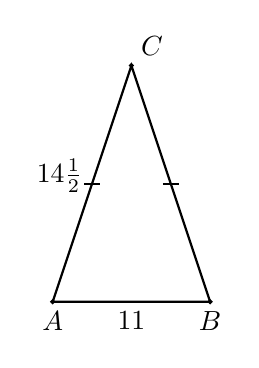
\begin{tikzpicture}[scale=0.5]
      \draw [thick](0,0)--(4,0)--(2,6)--(0,0);
      \draw [fill] (0,0) circle [radius=0.05] node[below]{$A$};
      \draw [fill] (4,0) circle [radius=0.05] node[below]{$B$};
      \draw [fill] (2,6) circle [radius=0.05] node[above right]{$C$};
      \draw [thick] (0.8,3)--(1.2,3); %tick mark
      \draw [thick] (2.8,3)--(3.2,3); %tick mark
      \node at (2,0) [below]{11};
      \node at (1,3.2) [left]{$14 \frac{1}{2}$};
    \end{tikzpicture}
  \end{frame}

\begin{frame}{Isosceles triangle perimeter}
Find the perimeter of the isosceles $\triangle ABC$, given $\overline{AC} \cong \overline{BC}$, $AB=7 \frac{1}{2}$, and $BC=11 \frac{3}{4}$\\[0.5cm]
    Show your work with an equation for full credit.\\
      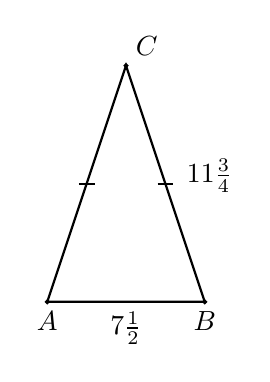
\begin{tikzpicture}[scale=0.5]
        \draw [thick](0,0)--(4,0)--(2,6)--(0,0);
        \draw [fill] (0,0) circle [radius=0.05] node[below]{$A$};
        \draw [fill] (4,0) circle [radius=0.05] node[below]{$B$};
        \draw [fill] (2,6) circle [radius=0.05] node[above right]{$C$};
        \draw [thick] (0.8,3)--(1.2,3); %tick mark
        \draw [thick] (2.8,3)--(3.2,3); %tick mark
        \node at (2,0) [below]{$7 \frac{1}{2}$};
        \node at (3.3,3.2) [right]{$11 \frac{3}{4}$};
      \end{tikzpicture}
    \end{frame}

\begin{frame}{Equilateral triangle}
  Given equilateral $\triangle ABC$ having perimeter of 21. Find the length of side $\overline{AB}$, $x$. \vspace{1cm}
  \begin{center}
  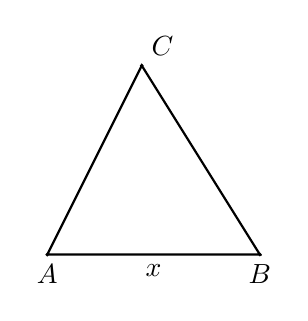
\begin{tikzpicture}[scale=0.3]
    \draw [thick](0,0)--(9,0)--(4,8)--(0,0);
    \draw [fill] (0,0) circle [radius=0.05] node[below]{$A$};
    \draw [fill] (9,0) circle [radius=0.05] node[below]{$B$};
    \draw [fill] (4,8) circle [radius=0.05] node[above right]{$C$};
    \node at (4.5,0) [below]{$x$};
  \end{tikzpicture}
  \end{center}
\end{frame}

\section{Extra: Circle definition }
\begin{frame}{Definition of a circle in a plane}
  A circle is defined by its center point and radius $r$ as\\
  all the points with distance $r$ to the center. \\[0.5cm]
  Shown below circle $C$, $\rm{radius}=2$\\[0.5cm]
    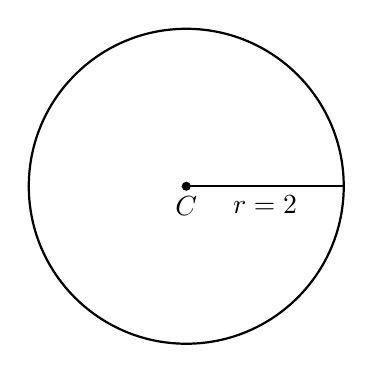
\begin{tikzpicture}
      \draw [-, thick] (0,0)--(2,0);
      \draw [thick] (0,0) circle [radius=2.0] node[below]{$C$};
      \draw [fill] (0,0) circle [radius=0.05];
      \node at (1,0) [below]{$r = 2$};
    \end{tikzpicture}\\
  Note: All of the radii of a circle are congruent.
    \end{frame}
  
\begin{frame}{Circle diagrams and notation}
  In circle $O$, which radius is longer? $\overline{OB}$ or $\overline{OC}$
  \begin{enumerate}
    \item $OB > OC$
    \item $OB < OC$
    \item $OB = OC$
    \end{enumerate}
    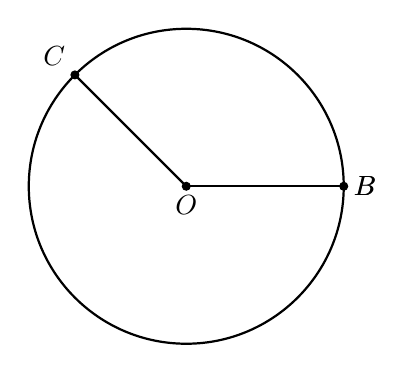
\begin{tikzpicture}
      \draw [-, thick] (0,0)--(2,0) node [right]{$B$};
      \draw [-, thick] (0,0)--(135:2);
      \draw [thick] (0,0) circle [radius=2.0];
      \draw [fill] (0,0) circle [radius=0.05] node[below]{$O$};
      \draw [fill] (2,0) circle [radius=0.05] node[right]{$B$};
      \draw [fill] (135:2) circle [radius=0.05] node[above left]{$C$};
      %\node at (1,0) [below]{$r = 2$};
    \end{tikzpicture}
\end{frame}


\section{Extra Trisect line segment }
\begin{frame}{Definition: Trisection of a line segment}
    Two points \emph{trisect} a line segment if they divide it into three congruent segments\\[1cm]
    Given $\overline{ABCD}$ with trisecting points $B$ and $C$. If $AD=9$, find ${x}$.\\[1cm]
    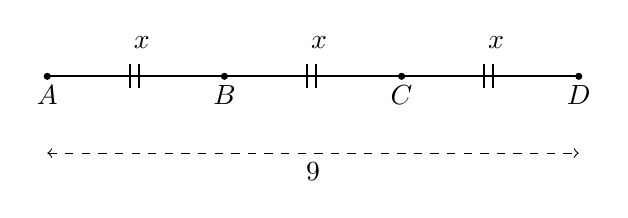
\begin{tikzpicture}[scale=0.75]
      \draw [-, thick] (0,0)--(9,0);
      \draw [fill] (0,0) circle [radius=0.05] node[below]{$A$};
      \draw [fill] (3,0) circle [radius=0.05] node[below]{$B$};
      \draw [fill] (6,0) circle [radius=0.05] node[below]{$C$};
      \draw [fill] (9,0) circle [radius=0.05] node[below]{$D$};
      \node at (1.6,0.3) [above]{$x$};
      \node at (4.6,0.3) [above]{$x$};
      \node at (7.6,0.3) [above]{$x$};
      \draw [-, thick] (1.4,-0.2)--(1.4,0.2);
      \draw [-, thick] (1.55,-0.2)--(1.55,0.2);
      \draw [-, thick] (4.4,-0.2)--(4.4,0.2);
      \draw [-, thick] (4.55,-0.2)--(4.55,0.2);
      \draw [-, thick] (7.4,-0.2)--(7.4,0.2);
      \draw [-, thick] (7.55,-0.2)--(7.55,0.2);
      \draw [<->, dashed] (0,-1.3)--(9,-1.3);
      \node at (4.5,-1.3) [below]{$9$};
    \end{tikzpicture} \vspace{1cm}
      \end{frame}

\begin{frame}{Segment trisection}
  The points $Q$ and $R$ trisect the line segment $\overline{PS}$. $PS=13 \frac{1}{2}$.
  \begin{enumerate}
    \item Mark and label the approximate locations of $Q$ and $R$.
    \item Find ${PQ}$. State an equation for full credit.
  \end{enumerate} \vspace{1cm} 
  \begin{center}
    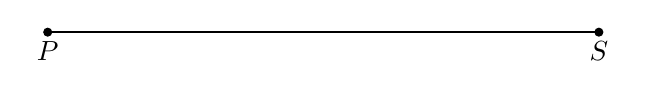
\begin{tikzpicture}
      \draw [-, thick] (0,0)--(7,0);
      \draw [fill] (0,0) circle [radius=0.05] node[below]{$P$};
      \draw [fill] (7,0) circle [radius=0.05] node[below]{$S$};
    \end{tikzpicture} 
  \end{center} \vspace{3cm} 
  \end{frame} 

  \begin{frame}{Segment trisection, find endpoint (spicy)}
      Given the points $S$ and $T$ trisect the line segment $\overline{RU}$, as shown below. If $SU=6$, find $RU$.\\[1cm]
      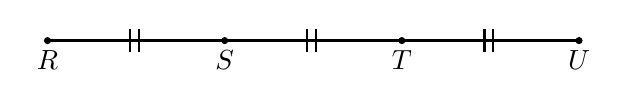
\begin{tikzpicture}[scale=0.75]
       \draw [-, thick] (0,0)--(9,0);
       \draw [fill] (0,0) circle [radius=0.05] node[below]{$R$};
       \draw [fill] (3,0) circle [radius=0.05] node[below]{$S$};
       \draw [fill] (6,0) circle [radius=0.05] node[below]{$T$};
       \draw [fill] (9,0) circle [radius=0.05] node[below]{$U$};
       %\node at (1.6,0.3) [above]{$x$};
       %\node at (4.6,0.3) [above]{$x$};
       %\node at (7.6,0.3) [above]{$x$};
       \draw [-, thick] (1.4,-0.2)--(1.4,0.2);
       \draw [-, thick] (1.55,-0.2)--(1.55,0.2);
       \draw [-, thick] (4.4,-0.2)--(4.4,0.2);
       \draw [-, thick] (4.55,-0.2)--(4.55,0.2);
       \draw [-, thick] (7.4,-0.2)--(7.4,0.2);
       \draw [-, thick] (7.55,-0.2)--(7.55,0.2);
       %\draw [<->, dashed] (0,-1.3)--(9,-1.3);
       %\node at (4.5,-1.3) [below]{$15$};
     \end{tikzpicture} \vspace{3cm}
    \end{frame} 

\section{Extra: Segment addition }
\begin{frame}{Applying the segment addition postulate}
  Given $\overline{LMN}$, $LM=2x+2$, $MN=15$, $LN=23$. Find ${x}$.
  \begin{center}
      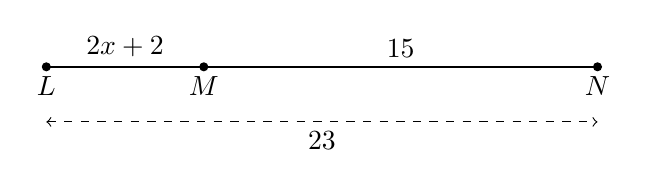
\begin{tikzpicture}
      \draw [-, thick] (0,0)--(7,0);
      \draw [fill] (0,0) circle [radius=0.05] node[below]{$L$};
      \draw [fill] (2,0) circle [radius=0.05] node[below]{$M$};
      \draw [fill] (7,0) circle [radius=0.05] node[below]{$N$};
      \node at (1,0) [above]{$2x+2$};
      \node at (4.5,0) [above]{$15$};
      \draw [<->, dashed] (0,-0.7)--(7,-0.7);
      \node at (3.5,-0.7) [below]{$23$};
    \end{tikzpicture}
  \end{center}
\begin{enumerate}
    \item Write down an equation to represent the situation. \vspace{0.5cm}
    \item Solve for $x$. \vspace{2cm}
    \item Check your answer. \vspace{2cm}
  \end{enumerate}
  \end{frame}
    
\begin{frame}{Find endpoint given bisector (spicy)}
  Given $S(1)$ and $T(3)$, as shown on the number line. \\[0.25cm]
  Find point $U$ given that point $T$ bisects $\overline{SU}$. Plot and label $U$ on the number line.\\[0.5cm]
    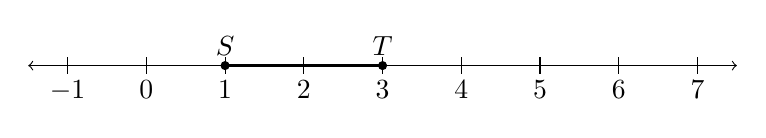
\begin{tikzpicture}
      \draw [<->] (-1.5,0)--(7.5,0);
      \draw [-, thick] (1,0)--(3,0);
      \foreach \x in {-1,...,7} %2 leading for diff!=1
        \draw[shift={(\x,0)},color=black] (0pt,-3pt) -- (0pt,3pt) node[below=5pt]  {$\x$};
        \draw [fill] (1,0) circle [radius=0.05] node[above] {$S$};
        \draw [fill] (3,0) circle [radius=0.05] node[above] {$T$};
    \end{tikzpicture} \vspace{4cm} 
\end{frame}

\end{document}